\documentclass[10pt]{beamer}

\usetheme[background=dark, numbering=fraction]{metropolis}
\usepackage{appendixnumberbeamer}
\usepackage{color, xcolor}
\usepackage{dsfont}
\definecolor{mydarkblue}{rgb}{0,0.08,0.45}
\usepackage{wrapfig}

\usepackage{booktabs}
\usepackage[scale=2]{ccicons}


\usepackage{adjustbox} 
\usepackage{pgfplots}
\usepgfplotslibrary{dateplot}
\usepackage{fourier-orns}
\usepackage{xspace}

\usepackage[scale=2]{ccicons}
\usepackage{fontawesome}


\usepackage[backend=bibtex,style=authoryear]{biblatex}
\addbibresource{index.bib}
\renewcommand*{\bibfont}{\scriptsize}
\let\oldcite=\cite                                                              
\renewcommand{\cite}[1]{\textcolor[rgb]{.7,.7,.7}{\oldcite{#1}}}
\let\oldparencite=\parencite                                                         
\renewcommand{\parencite}[1]{\textcolor[rgb]{.7,.7,.7}{\oldparencite{#1}}}


\newcommand{\themename}{\textbf{\textsc{metropolis}}\xspace}
% \DeclareMathOperator*{\argmin}{arg\,min}
% \DeclareMathOperator*{\minimize}{minimize}
% \DeclareMathOperator*{\maximize}{maximize}

\makeatletter
\renewcommand{\metropolis@colors@dark}{%
  \setbeamercolor{normal text}{%
    fg=black!2,
    bg=mDarkTeal
  }%
  \usebeamercolor[fg]{normal text}%
}
\renewcommand{\metropolis@colors@light}{%
  \setbeamercolor{normal text}{%
    fg=mDarkTeal,
    bg=black!2
  }%
  \usebeamercolor[fg]{normal text}%
}
\makeatother

\usepackage{tikz}
\usetikzlibrary{matrix,chains,positioning,decorations.pathreplacing,arrows}


\title{\huge Parallel Optimization in Machine Learning}
\author{
\large{\bfseries Fabian Pedregosa}}
% {\normalsize{ includes work with Remi Leblond and Simon Lacoste-Julien}}}
% \author{
% \hspace{4.8em}\includegraphics[width=0.2\linewidth]{img/remi}
% \hspace{4.8em}\includegraphics[width=0.2\linewidth]{img/SLJ}
% }\\
% {\normalsize\vphantom{}\hspace{0.5em} Fabian Pedregosa \hspace{3.5em} R\'emi Leblond \hspace{2.2em} Simon Lacoste--Julien}\\
% \vphantom{}\\
% \vphantom{}\includegraphics[width=0.3\linewidth]{img/logo_inria}
% \includegraphics[width=0.12\linewidth]{img/ens.png}
% \hspace{0.5em}\includegraphics[width=0.3\linewidth]{img/montreal}
% \hspace{0.5em}\includegraphics[width=0.2\linewidth]{img/mila}
% }
% 
\institute{

{\centerline{\hspace{2em}\includegraphics[width=0.3\linewidth]{img/Berkeley_wordmark_gold_no_uc}\hspace*{2em}
\includegraphics[width=0.3\linewidth]{img/eth_logo_kurz_neg}\hspace*{2em}
{\includegraphics[width=0.25\linewidth]{img/eu}}
}}
}
%\titlegraphic{\hfill\includegraphics[height=1.5cm]{figures/UCBerkeley_wordmark_blue.eps}}
\date{\vspace{1em}\today~{Huawei Paris Research Center}}

\input defs.tex



\begin{document}

\maketitle

\metroset{background=light} % change background theme according to manual
{
\usebackgroundtemplate{%
\begin{picture}(40,260)
  \includegraphics[height=0.9\paperheight]{img/white-rabbit}
  \end{picture}
  }
\begin{frame}{About me}
\begin{columns}
\begin{column}{0.4\textwidth}  %%<--- here
\end{column}
\begin{column}{0.6\textwidth}  %%<--- here
\begin{itemize}
\item Engineer (2010-2012), Inria Saclay (scikit-learn kickstart).
\item PhD (2012-2015, Inria Saclay)
\item Postdoc (2015-2016), Dauphine--ENS--Inria Paris.
\item Postdoc (2017-present), UC Berkeley - ETH Zurich (Marie-Curie fellowship, European Commission)
\end{itemize}
\end{column}
\end{columns}

\note{I should start by presenting myself. I started my career as an engineer }

\end{frame}
}

\metroset{background=dark} % change background theme according to manual

\begin{frame}{Motivation}
\begin{columns}[T] % align columns
\begin{column}{.5\textwidth}
\centering{Computer add in 1993}
\includegraphics[width=1.05\linewidth]{img/old_ad}
\end{column}%
\hfill%
\begin{column}{.5\textwidth}
\centering{Computer add in 2006}
\includegraphics[width=\linewidth]{img/2006_ad}
\end{column}%
\end{columns}
What has changed?
\pause
2006 = no longer mentions to speed of processors
\end{frame}


\begin{frame}{Moore's law}
\begin{quote}
The complexity for minimum component costs 
has increased at a rate of roughly a factor of 
two per year. Certainly over the short term this 
rate can be expected to continue
\end{quote}
Gordon Moore (Intel), 1965

\hspace{1em}\begin{quote}
OK, maybe a factor of two every two 
years.
\end{quote}
Gordon Moore (Intel), 1975 [paraphrased]
\end{frame}


\begin{frame}{40 years of CPU trends}
\centering\includegraphics[width=0.8\linewidth]{img/moore_law}

\begin{itemize}[<+->]
\item Speed of CPUs has stagnated since 2005;
\item Multi-core architectures are here to stay.
\end{itemize}
\pause {\bfseries Parallel algorithms needed to take advantage of modern CPUs.}
\end{frame}


% \begin{frame}{Outline}
% 
% {\bfseries Goal of the talk:} overview and state of the art in parallel optimization methods in machine learning.
% \end{frame}




\begin{frame}{Parallel optimization}
Parallel algorithms can be divided  into two large categories: 
{\bfseries synchronous} and {\bfseries asynchronous}.

\begin{figure}
\vspace{-1em}\begin{flushright}\vspace{-1em}{\scriptsize Image credits: \parencite{peng2016arock}}\end{flushright}
\vspace{-0.5em}\includegraphics[width=0.8\linewidth]{img/sync_vs_async}
\vspace{-0.5em}\end{figure}


\begin{columns}[T] % align columns
\begin{column}{.5\textwidth}
{\centering \bfseries Synchronous methods}

\vspace{0.5em}
~\faCheck~Easy to implement (i.e., developed software packages).

\vspace{0.5em}
~\faCheck~Well understood.

\vspace{0.5em}
~\faClose~Limited speedup due to synchronization costs..
\end{column}
\begin{column}{.5\textwidth}
{\centering \bfseries Asynchronous methods}

\vspace{0.5em}
~\faCheck~Faster, typically larger speedups.

\vspace{0.5em}
~\faClose~Not well understood, large gap between theory and practice.

\vspace{0.5em}
~\faClose~No mature software solutions.

\end{column}%
\end{columns}

\end{frame}



\begin{frame}{Outline}

{\centering \bfseries Synchronous methods}
\begin{itemize}
\item Synchronous (stochastic) gradient descent.
\end{itemize}
{\centering \bfseries Asynchronous methods}
\begin{itemize}
\item Asynchronous SGD (Hogwild)~\parencite{hogwild2011}
\item Asynchronous variance-reduced stochastic methods~\parencite{leblond2016Asaga}, \parencite{pedregosa2017proxasaga}.
\item Analysis of asynchronous methods. 
\item Codes and implementation aspects.
\end{itemize}

Leaving out many parallel synchronous methods: ADMM~\parencite{glowinski1975approximation}, CoCoA~\parencite{NIPS2014_5599}, DANE~\parencite{shamir2014communication}, to name a few.

\end{frame}

\begin{frame}{Outline}
Most of this is joint work with Remi Leblond and Simon Lacoste-Julien

{
% \hspace{1.8em}\includegraphics[width=0.2\linewidth]{img/fabian}
\hspace{4.8em}\includegraphics[width=0.2\linewidth]{img/remi}
\hspace{4.8em}\includegraphics[width=0.2\linewidth]{img/SLJ}
}\\
{\normalsize\vphantom{}
% \hspace{0.5em} Fabian Pedregosa
\hspace{4em} R\'emi Leblond \hspace{3em} Simon Lacoste--Julien}\\
% \vphantom{}\\
% \vphantom{}\includegraphics[width=0.3\linewidth]{img/logo_inria}
% \includegraphics[width=0.12\linewidth]{img/ens.png}
% \hspace{0.5em}\includegraphics[width=0.3\linewidth]{img/montreal}
% \hspace{0.5em}\includegraphics[width=0.2\linewidth]{img/mila}

\end{frame}


\section{Synchronous algorithms}

\begin{frame}{Optimization for machine learning}
Large part of problems in machine learning can be framed as optimization problems of the form
$$\minimize_x f(x) \defas \displaystyle\frac{1}{n}\sum^{n}_{i=1} f_i(x)$$
\begin{columns}
\begin{column}{0.6\textwidth}  %%<--- here
{\bfseries Gradient descent} \parencite{cauchy1847methode}. Descend along steepest direction ($-\nabla f(x)$)
$$x^+ = x - \gamma \nabla f(x)$$

{\bfseries Stochastic gradient descent} (SGD) \parencite{robbins1951sgd}. Select a random index $i$ and descent along $~\nabla f_i(x)$:
$$x^+ = x - \gamma \nabla f_i(x)$$

\end{column}
\begin{column}{0.4\textwidth}  %%<--- here
\includegraphics[width=\linewidth]{img/gd}

\vspace{2em}
\includegraphics[width=\linewidth]{img/sgd}
\vspace*{-2.5em}\begin{flushright}{\footnotesize images source: Francis Bach}\end{flushright}
\end{column}
\end{columns}
\end{frame}




\begin{frame}{Parallel synchronous gradient descent}

Computation of gradient is distributed among $k$ workers

\begin{figure}
{\centering\includegraphics[width=0.5\linewidth]{img/mapreduce}}
\end{figure}

\begin{columns}
\begin{column}{0.7\textwidth}  %%<--- here
\begin{itemize}
\item Workers can be: different computers, CPUs or GPUs

\item Popular frameworks: Spark, Hadoop.
\end{itemize}
\end{column}
\begin{column}{0.3\textwidth}  %%<--- here
\includegraphics[width=\linewidth]{img/gpu}
\end{column}
\end{columns}
\end{frame}


\begin{frame}{Parallel synchronous gradient descent}

% {\bfseries Idea:} Parallelize computation of $\nabla f(\xx)$ .

\begin{enumerate}
\item Choose $n_1, \ldots n_k$ that sum to $n$.
\item Distribute computation of $\nabla f(\xx)$ among $k$ nodes
\begin{align*}
\nabla f(\xx) &= \frac{1}{n} \sum_{i=1} \nabla f_i(\xx)\\ &= \frac{1}{k} \large(\underbrace{\frac{1}{n_1}\sum_{i=1}^{n_1} \nabla f_i(\xx)}_{\text{compute this in worker 1}} + \ldots + \underbrace{\frac{1}{n_1}\sum_{i=n_{k-1}}^{n_k} \nabla f_i(\xx)}_{\text{compute this in worker $k$}} \large)
\end{align*}
% {\centering\includegraphics[width=0.5\linewidth]{img/mapredu
\item Perform the gradient descent update by a master node
$$
\xx^+ = \xx - \gamma \nabla f(\xx)
$$
\end{enumerate}
\pause
\faCheck~Trivial parallelization, same analysis as gradient descent.
\faClose~Synchronization step every iteration (3.).
\end{frame}

\begin{frame}{Parallel synchronous SGD}
Can also be extended to stochastic gradient descent.
\begin{enumerate}
\item Select $k$ samples $i_{0}, \ldots, i_{k}$ uniformly at random.
\item Compute in parallel $\nabla f_{i_t}$ on worker $t$
\item Perform the (mini-batch) stochastic gradient descent update
$$
\xx^+ = \xx - \gamma \frac{1}{k}\sum_{t=1}^k \nabla f_{i_t}(\xx)
$$
\end{enumerate}
\pause
\faCheck~Trivial parallelization, same analysis as (mini-batch) stochastic gradient descent.

\faClose~Synchronization step every iteration (3.).
% This is the parallelization implemented in deep learning software: Tensorflow, PyTorch, etc.
\end{frame}

\section{Asynchronous algorithms}

\begin{frame}{Asynchronous SGD}

\begin{columns}
\begin{column}{0.5\textwidth}  %%<--- here
Synchronization is the bottleneck. \\

\vspace{1em}{\bfseries Idea:} What if we just ignore it?
\end{column}
\begin{column}{0.5\textwidth}  %%<--- here
\begin{center}
\includegraphics[width=\linewidth]{img/synchronization}
\end{center}
\end{column}
\end{columns}

\pause
Hogwild~\parencite{hogwild2011}: each core runs SGD in parallel, without synchronization, and updates the same vector of coefficients.

{\bfseries In theory}: convergence under very strong assumptions.

{\bfseries In practice}: just works.

\end{frame}

\begin{frame}{Hogwild in more detail}


Each core follows the same procedure
\begin{enumerate}
\item Read the information from shared memory $\hat{\xx}$.
\item Sample $i \in \{1, \ldots, n\}$ uniformly at random.
\item Compute partial gradient $\nabla f_i(\hat{\xx})$.
\item Write the SGD update to shared memory $\xx = \xx - \gamma \nabla f_i(\hat{\xx})$.
\end{enumerate}
\pause
\begin{figure}
\centering\includegraphics[width=0.6\linewidth]{img/async_updates}
\end{figure}
\end{frame}

\begin{frame}{Hogwild is fast}

Hogwild can be very fast. 
But its still SGD...

\begin{figure}
\includegraphics[width=0.8\linewidth]{img/figure_comparison_hogwild}
\end{figure}

\begin{itemize}
\item With constant step size, bounces around the optimum.

\item With decreasing step size, slow convergence.
\end{itemize}
\end{frame}

% if you want some excitement ...
\section{(A glipse into the) Analysis of asynchronous methods}

\begin{frame}{Analysis of asynchronous methods}

Things become unpredictable in presence of asynchrony.


{\bfseries How to name the iterates?}

\begin{figure}
\vspace{-0.5em}\includegraphics[width=0.8\linewidth]{img/sync_vs_async}
\vspace{-0.5em}\end{figure}

\note{

Many of the things we are used to in classical optimization just break down in the presence of asynchrony. Suddenly, we need to start worrying for things that we used to give for granted. One these things is how to name things. It sounds silly but its true,  

}
\end{frame}



\begin{frame}{Naming scheme in Hogwild}

{\bfseries Simple, intuitive and wrong}

Each time a core has finished writing to shared memory, increment iteration counter.

$\iff$ $\hat{\xx}_t = (t+1)$-th succesfull update.

\vspace{1em}\faWarning~In this framework, the value of $\hat{\xx}_t$ and $i_t$ are not determined until the iteration has finished.

$\implies$ $\hat{\xx}_t$ and $i_t$  are not necessarily independent.

\end{frame}

\begin{frame}{Unbiased gradient estimate}
SGD-like algorithms crucially rely on the property that update is unbiased estimate of the gradient, i.e., $\mathbb{E}_i[\nabla f_i(\xx)] = \nabla f(\xx)$.

For synchronous algorithms, this follows from the uniform sampling of $i$ 
\begin{align*}
\mathbb{E}_i[\nabla f_i(\xx)] &= \sum_{i=1}^n \text{Proba}(\text{selecting}~i) \nabla f_i(\xx)\\
 &\stackrel{\text{uniform sampling}}{=} \sum_{i=1}^n \frac{1}{n} \nabla f_i(\xx) = \nabla f(\xx)
\end{align*}
\end{frame}

\begin{frame}{A problematic example}

Selecting $i$ uniformly at random is not enough. 

\pause
{\bfseries Illustration}: problem with two samples and two cores $f = \frac{1}{2}(f_1 + f_2)$. Computing $\nabla f_1$ is much expensive than $\nabla f_2$.

Start at $\xx_0$. Because of the random sampling there are 4 possible scenarios:
\begin{enumerate}
\item Core 1 selects $f_1$, Core 2 selects $f_1$ $\implies$ $\xx_1 = \xx_0 - \nabla f_1(\xx)$
\item Core 1 selects $f_1$, Core 2 selects $f_2$ $\implies$ $\xx_1 = \xx_0 - \nabla f_2(\xx)$
\item Core 1 selects $f_2$, Core 2 selects $f_1$ $\implies$ $\xx_1 = \xx_0 - \nabla f_2(\xx)$
\item Core 1 selects $f_2$, Core 2 selects $f_2$ $\implies$ $\xx_1 = \xx_0 - \nabla f_2(\xx)$
\end{enumerate}
So we have
\begin{align*}
\mathbb{E}_i\left[\nabla f_i\right] &= \frac{1}{4}f_1 + \frac{3}{4} f_2 \\
&\neq \frac{1}{2}f_1 + \frac{1}{2} f_2 ~!!
\end{align*}
\end{frame}

\section{The Art of Naming Things}

\begin{frame}{The art of naming things}

{\bfseries Solution}: change the way we name iterates.

\pause
``After read'' labeling~\parencite{leblond2016Asaga}. Increment counter each time we \emph{read} the vector of coefficients from shared memory.

\faCheck~No dependency between $i_t$ and the cost of computing $\nabla f_{i_t}$.

Full (hopefully correct) analysis of Hogwild and other asynchronous methods in \emph{``Improved parallel stochastic optimization analysis for
incremental methods'', Leblond, P., and Lacoste-Julien} (submitted).
\end{frame}

\begin{frame}{Analysis}
Analysis inspired by the perturbed iterate framework of \parencite{mania2015perturbed}. Distinguishes two quantities:
\begin{itemize}
\item $\hat{\xx}_t =$ $(t+1)$-th fully completed read from shared memory. 
\item $\xx_{t+1} \defas \xx_{t} - \gamma \nabla f_i(\hat{\xx}_t)$
\end{itemize}

\end{frame}

\section{Asynchronous SAGA}


\begin{frame}{The SAGA algorithm}

{\bfseries Setting:}
$$
\minimize_x \frac{1}{n} \sum_{i=1}^n f_i(\xx)
$$ 

The {\bfseries SAGA} algorithm~\parencite{defazio2014saga}.

Select $i \in \{1, \ldots, n\}$ and compute $(\xx^+, \balpha^+)$ as
$$
\xx^+ = \xx - \gamma (\nabla f(\xx) - \balpha_i + \overline{\balpha})\,;~\balpha_i^+ = \nabla f_i(\xx)
$$
Unlike SGD, stores previous gradients ($\balpha$).
\vspace{1em}\pause
{\bfseries Motivation}: Can we derive an asynchronous parallel variant of this algorithm?
\end{frame}


\begin{frame}{X}
\end{frame}

\section{Asynchronous Proximal SAGA}



\begin{frame}{Composite objective}

\faExclamationTriangle~These methods assume objective function is smooth

Cannot be applied to Lasso, Group Lasso, box constraints, etc.

\pause 
\vspace{5mm}
{\bfseries Objective}: minimize composite objective function:
$$
\minimize_{\xx} f(\xx) + h(\xx)~,~ \text{ with $f(x) = \textstyle \frac{1}{n}\sum_{i=1}^n f_i(\xx)$}
$$
where $f_i$ is smooth and $h$ is a block-separable (i.e., $h(\boldsymbol{x}) = \sum_{B} h([\boldsymbol{x}]_B)$) convex function for which we have access to its proximal operator.
\end{frame}



% \begin{frame}{Sparse Proximal SAGA}
% 
% {\bfseries Contribution 1: Sparse Proximal SAGA.} Variant of SAGA \parencite{defazio2014saga}, particularly efficient when $\nabla f_i$ are sparse.
% % \vspace{0.5em}\begin{equation*}\tag{SAGA}
% % \xx^+ = \prox_{\gamma h}(\xx - \gamma (\nabla f_i(\xx) - \balpha_i + \overline{\balpha}))\,;~\balpha_i^+ = \nabla f_i(\xx)~.
% % \end{equation*}
% 
% % \begin{align}
% %     \vphantom{\sum}\vv_i &= \nabla f_i(\xx) - \balpha_i + \tikzmarkin<2>{a}\DD_i\tikzmarkend{a} \overline{\balpha}\,\\
% %     \vphantom{\sum}\xx^+ &= \prox_{\gamma \varphi_i}\big(\xx - \gamma \vv_i \big)\,;~
% %     \balpha_i^+ = \nabla f_i(\xx)
% % \end{align}
% 
% \onslide<2->{Like SAGA, it relies on \rnode{a}{unbiased gradient} estimate} \onslide<3->{ and \rnode{b}{proximal step}}
% 
% % \[
% % \onslide<2->{
% %       \vv_i \rnode[t]{ae}{=} \nabla f_i(\xx) - \balpha_i + \DD_i \overline{\balpha}\,; }
% % \onslide<3->{%
% %   ~\xx^+ = \rnode[t]{be}{\prox}_{\gamma \varphi_i}(\xx - \gamma \vv_i)\,;~\balpha_i^+ = \nabla f_i(\xx)}
% % \] 
% %  \onslide<2->{\nccurve[angleA=-90,angleB=90, linecolor=gray]{->}{a}{ae}}
% %  \onslide<3->{\nccurve[angleA=-90, angleB=90, linecolor=gray]{->}{b}{be}}
%  
%  \onslide<4->{
%  {Unlike SAGA}, and $\varphi_i$ are designed to give sparse updates while verifying unbiasedness conditions.}
%  
% \onslide<5->{ {\bfseries Convergence:} same linear convergence rate as SAGA, with cheaper updates in presence of sparsity. 
%  }
% \end{frame}


\begin{frame}{Proximal Asynchronous SAGA (ProxASAGA)}

{\bfseries Contribution 2: Proximal Asynchronous SAGA (ProxASAGA).} Each core
 runs Sparse Proximal SAGA asynchronously without locks and updates $\xx$, $\balpha$ and $\overline{\balpha}$ in shared memory.

\vspace{0.5em} \faRandom~All read/write operations to shared memory are \emph{inconsistent}, i.e., no performance destroying vector-level locks while reading/writing.

{\bfseries Convergence:} under sparsity assumptions, ProxASAGA converges with the same rate as the sequential algorithm $\implies$ theoretical linear speedup with respect to the number of cores.
\end{frame}


\begin{frame}{Empirical results}



% \begin{columns}[T] % align columns
% \begin{column}{.35\textwidth}
% \end{column}%
% \hfill%
% \begin{column}{.65\textwidth}
% \includegraphics[width=1\linewidth]{img/prox_asaga_1}
% \end{column}%
% \end{columns}

ProxASAGA vs competing methods on 3 large-scale datasets, $\ell_1$-regularized logistic regression

\vspace{0em}\begingroup
\fontsize{9pt}{10pt}\selectfont
\begin{table}
\centering
%\resizebox{\linewidth}{!}{
\begin{tabular}{lrrrrr}
\toprule
{\bfseries\sffamily Dataset} & \multicolumn{1}{c}{$n$} & \multicolumn{1}{c}{$p$} & {{density}} & \multicolumn{1}{c}{$L$} & $\Delta$\\
\midrule
{\bfseries\sffamily KDD 2010} & \hfill 19,264,097 & \hfill 1,163,024 & \hfill $10^{-6}$ & \hfill 28.12 & 0.15\\
{\bfseries\sffamily KDD 2012} & \hfill 149,639,105 & \hfill 54,686,452 & \hfill $2 \times 10^{-7}$ & \hfill $1.25$ & 0.85\\
{\bfseries\sffamily Criteo} & \hfill 45,840,617 & \hfill 1,000,000 & \hfill $4 \times 10^{-5}$ & \hfill $1.25$ & 0.89\\
\bottomrule
\end{tabular}
%}
%\vspace{-5mm}
\end{table}
\endgroup


\includegraphics[width=1\linewidth]{img/prox_asaga_1}

\end{frame}


\begin{frame}{Empirical results - Speedup}

$$
\text{Speedup} = \frac{\text{Time to $10^{-10}$ suboptimality 
on one core}}{\text{Time to same suboptimality on $k$ cores}}
$$

\includegraphics[width=\linewidth]{img/prox_asaga_2}

\begin{itemize}
\pause \item ProxASAGA achieves speedups between 6x and 12x on a 20 cores architecture.

\pause \vspace{0.5em}\item As predicted by theory, there is a high correlation between degree of sparsity and speedup.
\end{itemize}

\pause Thanks for your attention, see you at {\bfseries poster \#159}.
\end{frame}

\begin{frame}{XX}

\faGithub~Code is in github: \url{https://github.com/fabianp/ProxASAGA}

A very efficient implementation of SAGA can be found in scikit-learn
\end{frame}



\begin{frame}{Supervised Machine Learning}

{\bfseries Data}: $n$ observations $(\boldsymbol{a}_i, b_i) \in \mathbb{R}^p \times \mathbb{R}$

{\bfseries Prediction function}: $h(\boldsymbol{a}, \boldsymbol{x}) \in \RR$


{\bfseries Motivating examples:}
\begin{itemize}
\item Linear prediction: $h(\boldsymbol{a}, \xx) = \xx^T\boldsymbol{a}$
\item Neural networks: $h(\boldsymbol{a}, \xx) = \xx_m^T \sigma(\xx_{m-1}\sigma(\cdots\xx_2^T\sigma(\xx_1^T\boldsymbol{a}))$
\end{itemize}

\only<1>{
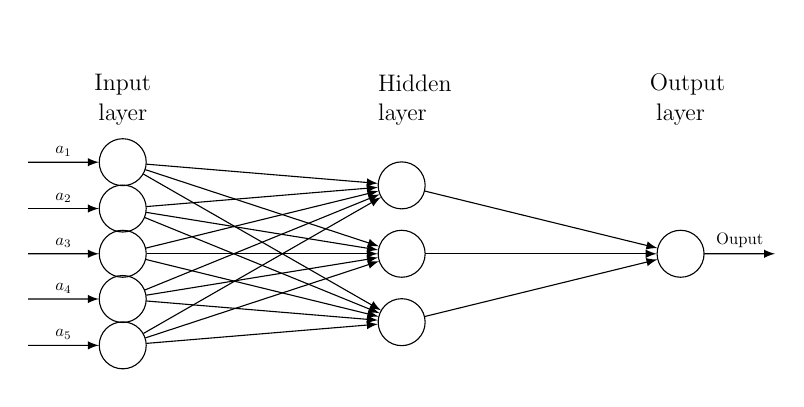
\begin{tikzpicture}[
ampersand replacement=\&,
scale=0.6,
every node/.style={scale=0.6},
plain/.style={
  draw=none,
  fill=none,
  },
net/.style={
  matrix of nodes,
  nodes={
    draw,
    circle,
    inner sep=10pt
    },
  nodes in empty cells,
  column sep=2cm,
  row sep=-9pt
  },
>=latex
]
\matrix[net] (mat)
{
|[plain]| \parbox{1.3cm}{\centering \Large Input\\layer} \& |[plain]| \parbox{1.0cm}{\centering\Large Hidden\\layer} \& |[plain]| \parbox{1.3cm}{\centering \Large Output\\layer} \\
\& |[plain]| \\
|[plain]| \& \\
\& |[plain]| \\
  |[plain]| \& |[plain]| \\
\& \& \\
  |[plain]| \& |[plain]| \\
\& |[plain]| \\
  |[plain]| \& \\
\& |[plain]| \\    };
\foreach \ai [count=\mi ]in {2,4,...,10}
  \draw[<-] (mat-\ai-1) -- node[above] {$\boldsymbol{a}_{\mi}$} +(-2cm,0);
\foreach \ai in {2,4,...,10}
{\foreach \aii in {3,6,9}
  \draw[->] (mat-\ai-1) -- (mat-\aii-2);
}
\foreach \ai in {3,6,9}
  \draw[->] (mat-\ai-2) -- (mat-6-3);
\draw[->] (mat-6-3) -- node[above] {Ouput} +(2cm,0);
\end{tikzpicture}
}
\only<2>{
{\bfseries Minimize some distance (e.g., quadratic) between the prediction}
$$
\minimize_{\xx} \frac{1}{n}\sum_{i=1}^n \ell(\boldsymbol{b}_i, h(\boldsymbol{a}_i, \xx)) \stackrel{\text{notation}}{=} \frac{1}{n}\sum_{i=1}^n f_i(\xx)
$$
where popular examples of $\ell$ are
\begin{itemize}
\item Squared loss, $ \ell(\boldsymbol{b}_i, h(\boldsymbol{a}_i, \xx)) \defas (\boldsymbol{b}_i - h(\boldsymbol{a}_i, \xx))^2$
\item Logistic (softmax), $ \ell(\boldsymbol{b}_i, h(\boldsymbol{a}_i, \xx)) \defas \log(1 + \exp(-\boldsymbol{b}_i h(\boldsymbol{a}_i, \xx)))$
\end{itemize}
}

\note{
The kind of parallelization will depend on the problem.
The kind of problem that we will be interested in
The problem: supervised learning.
}


\end{frame}




\begin{frame}[noframenumbering, allowframebreaks]
\nocite{pedregosa2017proxasaga}
  % \frametitle{References}
  \printbibliography
 \end{frame}

\end{document}
